\documentclass{beamer}

\usepackage{amsfonts,amsmath,oldgerm}
\usepackage{listings}
\usepackage{colortbl}
\usepackage{xcolor}
\usepackage{verbatim}
\usepackage{multicol}
\usepackage{subcaption}
\usepackage{etoolbox}
\usepackage{relsize}
\usepackage{ragged2e}

\makeatletter
\patchcmd{\itemize}{\raggedright}{\justifying}{}{}
\patchcmd{\beamer@enum@}{\raggedright}{\justifying}{}{}
\patchcmd{\@@description}{\raggedright}{\justifying}{}{}
\makeatother
\usepackage{microtype}
\usepackage{amsmath}
\usepackage[ruled,vlined]{algorithm2e}
\SetAlCapNameFnt{\scriptsize}
\SetAlCapFnt{\scriptsize}
\SetAlFnt{\scriptsize}

\usepackage{graphicx}
\usepackage[scale=2]{ccicons}
\usepackage{qrcode}
\usepackage{tikz}
\usepackage{tikzpagenodes}
\usetikzlibrary{positioning}

\usepackage{array}
\usepackage{booktabs}
\usepackage{multirow}
\usepackage{colortbl}
\newcommand{\tabincell}[2]{\begin{tabular}{@{}#1@{}}#2\end{tabular}}

\usepackage{minted}
\newminted{bash}{}
\newminted{latex}{}
\newmintinline{bash}{}
\newmintinline{latex}{}
\newcommand{\texdoc}[2]{\href{#2}{\bashinline|texdoc #1|}}


\usetheme{_statale}
\usefonttheme[onlymath]{serif}


\setbeamertemplate{caption}[numbered]
\newcommand{\testcolor}[1]{\colorbox{#1}{\textcolor{#1}{test}}~\texttt{#1}}
\newcommand{\hrefcol}[2]{\textcolor{frmtxt}{\href{#1}{#2}}}

% ==================///==================///==================///
% ==================/// Inicio
% ==================///==================///==================///


\setbeamertemplate{title page}{
    \begin{tikzpicture}[remember picture,overlay]
        \node[at=(current page.center)] {
            
\includegraphics[width=\paperwidth,height=\paperheight]{assets/cartelcharla.jpg}
        };
    \end{tikzpicture}
}

% ==================///==================///==================///
% ==================/// Comenzar presentación
% ==================///==================///==================///

\pgfplotsset{compat=1.18}
\usetikzlibrary{positioning}
\begin{document}
\maketitle



\input{Sections/Cómo usar LaTeX}
\input{Sections/Estructura básica}
\section{Formato avanzado}

\begin{frame}[fragile]{Sintaxis}
  \begin{itemize}
    \item El código de \LaTeX{} es texto plano.
    \item \LaTeX{} si hay varios espacios o un salto de línea, lo trata como un único espacio. \\
          IUna línea vacía crea un nuevo párrafo.
    \item \latexinline|\\| o \latexinline|\newline| provocan un salto de línea.
  \end{itemize}
\end{frame}

\begin{frame}[fragile]{Caracteres especiales}
  \begin{itemize}
    \item  Algunos caracteres están reservados.
          \begin{latexcode}
            \# \$ \% \^{} \& \_ \{ \} \~{}
            \textbackslash
          \end{latexcode}
    \item Guiones:
          \begin{itemize}
            \item \textbf{guion}: \latexinline|-|
            \item \textbf{signo menos}: \latexinline|-|
          \end{itemize}
    \item \latexinline|\ldots| para puntos suspensivos.
  \end{itemize}
\end{frame}

\begin{frame}[fragile]{Fuente y Tamaño}
  \begin{table}
    \centering
    \begin{tabular}{@{}>{\columncolor{mintedbg}}ll@{\qquad}>{\columncolor{mintedbg}}ll@{}}
      \latexinline|\textrm{...}|     & \textrm{romano}             &
      \latexinline|\textsf{...}|     & \textsf{sans serif}          \\
      \latexinline|\texttt{...}|     & \texttt{máquina de escribir}        &
                                     &                              \\
      \latexinline|\textmd{...}|     & \textmd{medio}            &
      \latexinline|\textbf{...}|     & \textbf{negrita}           \\
      \latexinline|\textup{...}|     & \textup{recto}           &
      \latexinline|\textit{...}|     & \textit{itálica}              \\
      \latexinline|\textsl{...}|     & \textsl{inclinado}           &
      \latexinline|\textsc{...}|     & \textsc{pequeñas mayúsculas}          \\
      \latexinline|\emph{...}|       & \emph{enfatizado}          &
      \latexinline|\textnormal{...}| & \textnormal{fuente del documento}
    \end{tabular}
    \caption{Comandos para tipo de fuente}
  \end{table}

  \begin{itemize}
    \item Si pones el texto como argumento, este cambiará. \\
          e.g.~\latexinline|\textbf{este texto estará en negrita}|
  \end{itemize}
\end{frame}

\begin{frame}[fragile]{Fuente y Tamaño}
  \begin{columns}
    \begin{column}{0.5\textwidth}
      \begin{table}
        \centering
        \begin{tabular}{@{}>{\columncolor{mintedbg}}ll}
          \latexinline|\tiny|         & {\tiny enano}                \\
          \latexinline|\scriptsize|   & {\scriptsize muy pequeño}    \\
          \latexinline|\footnotesize| & {\footnotesize bastante pequeño} \\
          \latexinline|\small|        & {\small pequeño}              \\
          \latexinline|\normalsize|   & {\normalsize normal}        \\
          \latexinline|\large|        & {\large grande}              \\
          \latexinline|\Large|        & {\Large grande}              \\
          \latexinline|\LARGE|        & {\LARGE muy grande}         \\
          \latexinline|\huge|         & {\huge enorme}                     \\
          \latexinline|\Huge|         & {\Huge gigante}
        \end{tabular}
        \caption{Comandos para tamaño Fuente}
      \end{table}
    \end{column}
    \begin{column}{0.5\textwidth}
      \begin{itemize}
        \item Los comandos afectarán al texto siguiente
        \item Usa \latexinline|{ ... }| para limitar su efecto   \\
              ~\latexinline|{\small texto pequeño}|
      \end{itemize}
    \end{column}
  \end{columns}

\end{frame}

\begin{frame}[fragile]{Espacio/Spacing}
  \begin{itemize}
    \item Usa el paquete geometry para cambiar los márgenes.
          \begin{latexcode}
            \usepackage[top=3cm,bottom=3cm,left=2.5cm,right=2.5cm]{geometry}
          \end{latexcode}
    \item Para crear una nueva página:
          \begin{itemize}
            \item \latexinline|\newpage|
          \end{itemize}
    \item Inserta espacios horizontales/verticales con \latexinline|\hspace{1em}| o \latexinline|\vspace{1ex}|
    \item Rellena espacio usando \latexinline|\hfill| o \latexinline|\vfill|
  \end{itemize}
\end{frame}


\begin{frame}[fragile]{Estructura del documento}
  \begin{itemize}
    \item La principal idea de \LaTeX  es el formato.
    \item Puedes estructurar los documentos con los siguientes comandos:
          \begin{latexcode}
            \part{parte} % solo disponible en book
            \chapter{capitulo} % solo disponible en book y report
            \section{seccion}
            \subsection{subseccion}
            \subsubsection{subsubseccion}
          \end{latexcode}
    \item \latexinline|\tableofcontents| se puede usar para crear una tabla de contenidos.
    \item Usa \latexinline|\appendix| para poner el resto del contenido en el apéndice.
    \item Para proyectos grandes, pon cada sección en un archivo. \\
          Luego usa \latexinline|\input{file_name}| para incluirlo en el archivo principal.
  \end{itemize}
\end{frame}

\begin{frame}[fragile]{Listas}
  \begin{itemize}
    \item Hay tres tipos de listas: Enumerate, itemize y description
          \begin{latexexample}
            \begin{enumerate}
              \item Item 1
              \item Item 2
            \end{enumerate}
            \begin{itemize}
              \item Item 1
              \item Item 2
            \end{itemize}
            \begin{description}
              \item[key1] Item 1
              \item[key2] Item 2
            \end{description}
          \end{latexexample}
  \end{itemize}
\end{frame}

\begin{frame}[fragile]{Listas}
  \begin{itemize}
    \item Se pueden anidar
          \begin{latexexample}
            \begin{enumerate}
              \item Nivel 1
                    \begin{enumerate}
                      \item Nivel 2
                    \end{enumerate}
              \item Nivel 1
                    \begin{itemize}
                      \item Nivel 2
                    \end{itemize}
            \end{enumerate}
          \end{latexexample}
  \end{itemize}
\end{frame}

\begin{frame}[fragile]{Matemáticas y ecuaciones/fórmulas}
  \begin{itemize}
    \item Algunos paquetes típicos para matemáticas
          \begin{latexcode}
            \usepackage{amsmath}
            \usepackage{amssymb}
            \usepackage{amsfonts}
            \usepackage{mathrsfs}
            \usepackage{latexsym}
          \end{latexcode}
    \item Lista de símbolos matemáticos \url{https://www.caam.rice.edu/~heinken/latex/symbols.pdf}
    \item Detexify: Herramienta para dibujar símbolos
    \url{https://detexify.kirelabs.org/classify.html}
  \end{itemize}
\end{frame}

\begin{frame}[fragile]{Modos de representar las matemáticas y entorno}
  \begin{itemize}
    \item Hay dos modos de representar fórmulas:
          \begin{itemize}
            \item  Dentro de línea (1 símbolo dolar): \latexinline|$\sum_k^n k$| o \latexinline|\(\sum_k^n k\)| para representar \(\sum_k^n k\)
            \item Exposición: \latexinline|$$\sum_k^n k$$| o \latexinline|\[\sum_k^n k\]| para representar
                  \[\sum_k^n k\]
          \end{itemize}
    \item Usa \latexinline|equation| para poder representar una ecuación
          \begin{latexexample}
            \begin{equation}
              E = mc^2
            \end{equation}
          \end{latexexample}
    \item Usa \latexinline|\tag| para cambiar la etiqueta de la ecuación.
          \begin{latexexample}
            \begin{equation}
              2 + 2 = 5 \tag{verdad}
            \end{equation}
          \end{latexexample}
  \end{itemize}
\end{frame}

\begin{frame}[fragile]{Modos de representar las matemáticas y entorno}
  \begin{itemize}
    \item Usa \latexinline|\align| para alinear varias ecuaciones.
          % \begin{noindent}
          \begin{latexexample}
            \begin{align}
              B' &=-\nabla \times E, \\
              E' &=\nabla \times B - 4\pi j,
            \end{align}
          \end{latexexample}
          % \end{noindent}
    \item Usa \latexinline|\nonumber| para deshabilitar la etiqueta con el número.
          % \begin{noindent}
          \begin{latexexample}
            \begin{align}
              a &= b + c \nonumber \\
                &= d + e
            \end{align}
          \end{latexexample}
          % \end{noindent}
  \end{itemize}
\end{frame}

\begin{frame}[fragile]{Modos de representar las matemáticas y entorno}
  \begin{itemize}
    \item \latexinline|\align*| deshabilita la etiqueta del número y alinea directamente.
          % \begin{noindent}
          \begin{latexexample}
            \begin{align*}
              B' &=-\nabla \times E, \\
              E' &=\nabla \times B - 4\pi j,
            \end{align*}
          \end{latexexample}
          % \end{noindent}
    \item \latexinline|\gather|/\latexinline|\gather*| muestra ecuaciones centradas pero sin alinear.
          % \begin{noindent}
          \begin{latexexample}
            \begin{gather*}
              2x - 5y =  8 \\
              3x^2 + 9y =  3a + c
            \end{gather*}
          \end{latexexample}
          % \end{noindent}
  \end{itemize}
\end{frame}

\begin{frame}[fragile]{Símbolos}
  \begin{itemize}
    \item Se pueden utilizar los siguientes símbolos:
          \begin{mathexamples}
            + - = ! / ( ) [ ] < > | ' : *
          \end{mathexamples}
    \item Letras griegas
          \begin{mathexamples}
            \alpha, \beta, \gamma, \pi, \phi, \varphi
          \end{mathexamples}
    \item Operadores
          \begin{mathexamples}
            \cos(2\theta) = \cos^2\theta-\sin^2\theta
            \lim\limits_{x \to \infty} \exp(-x) = 0
            a \bmod b
            x \equiv a \pmod{b}
            \log{(N)}
          \end{mathexamples}
  \end{itemize}
\end{frame}



\begin{frame}[fragile]{Potencias, Indices, Fracciones, Raíces}
  \begin{itemize}
    \item Se usa (\latexinline|^|) para elevar algo y la barra baja (\latexinline|_|) para subíndices u otros usos. Se deben usar (\latexinline|{| y \latexinline|}|) si hay más de un elemento.
          \begin{mathexamples}
            k_{n+1} = n^2 + k_n^2 - k_{n-1}
            n^{22}
            f(n) = n^5 + 4n^2 + 2 |_{n=17}
            \sum_{i=1}^{n} i
            \lim_{x \to \infty} \frac{1}{x}
          \end{mathexamples}
    \item Fracción con \latexinline|\frac| y raíz con \latexinline|\sqrt|
          \begin{mathexamples}
            \frac{n!}{k!(n-k)!} = \binom{n}{k}
            \sqrt{2}
            \sqrt[n]{1+x+x^2+x^3+\dots+x^n}
          \end{mathexamples}
  \end{itemize}
\end{frame}


\begin{frame}[fragile]{Matrices}
  \begin{itemize}
    \item Matrices \latexinline|\begin{matrix}|
          \begin{mathexample}
            \begin{matrix}
              a & b & c \\
              d & e & f \\
              g & h & i
            \end{matrix}
          \end{mathexample}
          \begin{mathexample}
            \begin{pmatrix}
              a & b & c \\
              d & e & f \\
              g & h & i
            \end{pmatrix}
          \end{mathexample}
    \item Otro tipo de matrices con otros entornos: \latexinline|bmatrix|, \latexinline|Bmatrix|, \latexinline|vmatrix|, and \latexinline|Vmatrix|
  \end{itemize}
\end{frame}

\begin{frame}[fragile]{Array}
  \begin{itemize}
    \item Array \latexinline|\begin{array}|
          \begin{mathexample}
            \begin{array}{c|c}
              1 & 2 \\
              \hline
              3 & 4
            \end{array}
          \end{mathexample}
          \begin{mathexample}
            f(x) = \left\{
            \begin{array}{ll}
              x & \text{si } x > 0, \\
              0 
            \end{array}\right.
          \end{mathexample}
    \item Casos \latexinline|\begin{cases}|
          \begin{mathexample}
            f(x) = \begin{cases}
              x & \text{si } x > 0, \\
              0 
            \end{cases}
          \end{mathexample}
  \end{itemize}
\end{frame}

\begin{frame}[fragile]{Fuentes para matemáticas}
  \begin{table}
    \begin{tabular}{>{\columncolor{mintedbg}}ll}
      \latexinline|\mathnormal{...}| & $\mathnormal{ABCDEF~abcdef~123456}$ \\
      \latexinline|\mathrm{...}|     & $\mathrm{ABCDEF~abcdef~123456}$     \\
      \latexinline|\mathit{...}|     & $\mathit{ABCDEF~abcdef~123456}$     \\
      \latexinline|\mathbf{...}|     & $\mathbf{ABCDEF~abcdef~123456}$     \\
      \latexinline|\mathsf{...}|     & $\mathsf{ABCDEF~abcdef~123456}$     \\
      \latexinline|\mathtt{...}|     & $\mathtt{ABCDEF~abcdef~123456}$     \\
      \latexinline|\mathfrak{...}|   & $\mathfrak{ABCDEF~abcdef~123456}$   \\
      \latexinline|\mathcal{...}|    & $\mathcal{ABCDEF}$                  \\
      \latexinline|\mathbb{...}|     & $\mathbb{ABCDEF}$
    \end{tabular}
    \caption{Fuentes para matemáticas}
  \end{table}
\end{frame}


\begin{frame}[fragile]{Gráficos/imágenes y tablas}
  \begin{itemize}
    \item Para crear un bloque para un gráfico, imagen o una tabla:
          \begin{latexcode}
            % gráfico
            \begin{figure} ... \end{figure}
            % tabla
            \begin{table} ... \end{table}
          \end{latexcode}
  \end{itemize}
\end{frame}

\begin{frame}[fragile]{Gráficos/imágenes y tablas}
  \begin{table}
    \small
    \begin{tabular}{lp{.8\linewidth}}
      \toprule
      \textbf{Especificador} & \textbf{Descripción}                                                                                                        \\
      \midrule
      h                  & Coloca el objeto flotante aquí, es decir, aproximadamente en el mismo punto en el que ocurre en el texto fuente (sin embargo, no exactamente en el lugar). \\
      t                  & Posición en la parte superior de la página.                                                                                          \\
      b                  &  Posición en la parte inferior de la página.                                                                                       \\
      p                  &Colocar en una página especial solo para objetos flotantes.                                                                                    \\
      !                  & Sobreescribe los parámetros internos que LaTeX utiliza para determinar las "buenas" posiciones de los objetos flotantes                                           \\
      H                  & Coloca el objeto flotante exactamente en la ubicación en el código LaTeX. \par Requiere  \latexinline|\usepackage{float}|.                \\
      \bottomrule
    \end{tabular}
    \caption{Especificador de posición para objetos flotantes}
  \end{table}

  \begin{itemize}
    \item Puedes usar uno o múltiples especificadores. 
  \end{itemize}
\end{frame}

\begin{frame}[fragile]{Gráfico/Imagen}
  \begin{itemize}
    \item Se requiere comúnmente el paquete \latexinline|\usepackage{graphicx}| para insertar un gráfico.
    \item Se pueden usar la mayoría de formatos.
  \end{itemize}
  \begin{figure}[b]
  \centering
  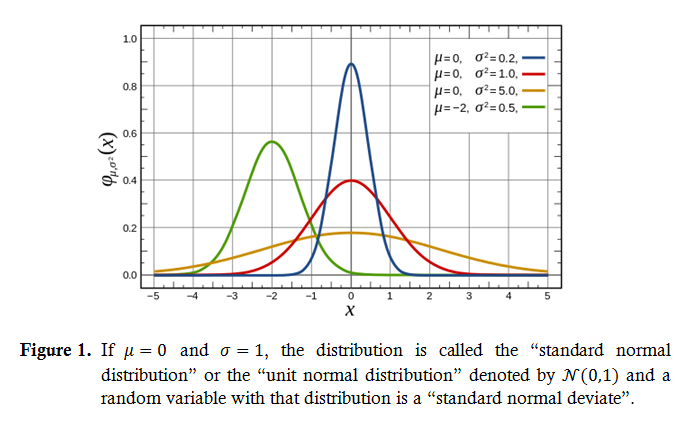
\includegraphics[width=0.8\textwidth, height=0.8\textheight, keepaspectratio]{assets/grafico.png}
  \end{figure}
\end{frame}


\begin{frame}[fragile]{Descripción (de imagen)}
  \begin{itemize}
    \item Usa \latexinline|\caption{}| y  \latexinline|\caption*{}| para que no esté numerado.
  \end{itemize}
\end{frame}

\begin{frame}[fragile]{Gŕafico/imagen}
  \begin{itemize}
    \item Ejemplo:
          \begin{latexcode}
            \begin{figure}[t] % parte superior
              \centering
              \includegraphics[width=.8\linewidth]{ruta_imagen}
              \caption{Descripción}
            \end{figure}
          \end{latexcode}
  \end{itemize}
\end{frame}


\begin{frame}[fragile]{Subflotantes}
  \begin{itemize}
    \item Usa el paquete \href{http://texdoc.net/texmf-dist/doc/latex/caption/subcaption.pdf}{\emph{subcaption}} para crear subfiguras (imágenes) o subtablas
          \begin{latexcode}
            \begin{figure}
              \centering
              \begin{subfigure}[b]{0.5\textwidth}
                \includegraphics[width=0.8\textwidth, height=0.8\textheight, keepaspectratio]{gato}
                \caption{Mi gato calcetines}
              \end{subfigure}
              \begin{subfigure}[b]{0.5\textwidth}
                \includegraphics[width=0.8\textwidth, height=0.8\textheight, keepaspectratio]{perro}
                \caption{Mi perro Toby}
              \end{subfigure}
              \caption{Fotos de mis mascotas}
            \end{figure}
          \end{latexcode}
  \end{itemize}
\end{frame}
\begin{frame}[fragile]{Subflotantes:ejemplo}
  \begin{figure}[b]
  \centering
  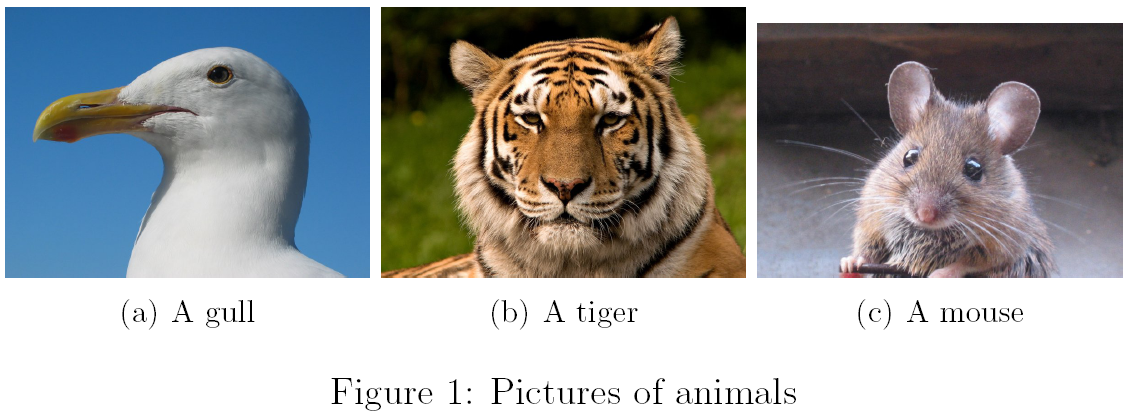
\includegraphics[width=0.8\textwidth, height=0.8\textheight, keepaspectratio]{assets/ejemplo2.png}
  \end{figure}
\end{frame}

\begin{frame}[fragile]{Referencias}
  \begin{itemize}
    \item Puedes usar \latexinline|\label{<label name>}| para crear una etiqueta
          \begin{latexcode*}{fontsize=\scriptsize}
            \section{Título sección}\label{sec:label-a}
            \begin{figure}
              ...
              \caption{subtítulo figura}\label{fig:label-b}
            \end{figure}
            \begin{equation}
              E=mc^2 \label{ecn:lable-c}
            \end{equation}
          \end{latexcode*}
    \item Usa \latexinline|\ref{<label name>}| para referenciarlo
    \item Con el paquete \href{http://texdoc.net/texmf-dist/doc/latex/hyperref/manual.pdf}{\emph{hyperref}} se puede crear una url ~\latexinline|\url{https://google.com}|
    \item Usa \latexinline|\footnote{...}| para el pie de página.
  \end{itemize}
\end{frame}



\begin{frame}[fragile]{Algoritmos}
  \begin{itemize}
    \item Se puede usar \emph{algorithm2e}:
    \item Ejemplo:
          \begin{latexexample}
            \begin{algorithm}[H]
              \caption{Como escribir algoritmos}
              \KwData{Datos}
              \KwResult{aprende a escribir un algoritmo}
              inicializacion\;
              \While{no termine el documento}{
                leer\;
                \eIf{entiende}{
                  go to siguiente seccion\;
                  current seccion se convierte en esta\;
                }{
                  volver al principio\;
                }
              }
            \end{algorithm}
          \end{latexexample}
  \end{itemize}
\end{frame}
\begin{frame}[fragile]{Algoritmos}
          \begin{latexcode}
            \begin{algorithm}[H]
              \caption{Como escribir algoritmos}
              \KwData{Datos}
              \KwResult{aprende a escribir un algoritmo}
              inicializacion\;
              \While{no termine el documento}{
                leer\;
                \eIf{entiende}{
                  go to siguiente seccion\;
                  current seccion se convierte en esta\;
                }{
                  volver al principio\;
                }
              }
            \end{algorithm}
          \end{latexcode}
\end{frame}

\begin{frame}[fragile]{Código}
  \begin{itemize}
    \item Se usa \href{http://texdoc.net/texmf-dist/doc/latex/listings/listings.pdf}{\emph{listings}} para escribir código fuente.
          % \begin{noindent}
        \begin{latexexample}
    \begin{lstlisting}[language=Python]
    def fib():
      a, b = 0, 1
      while 1:
        yield a
        a, b = b, a + b
    \end{lstlisting}
        \end{latexexample}
        \begin{latexcode}
            
    \begin{lstlisting}[language=Python]
    def fib():
      a, b = 0, 1
      while 1:
        yield a
        a, b = b, a + b
    \end{lstlisting}
        \end{latexcode}
  \end{itemize}
\end{frame}

\begin{frame}[fragile]{Bibliografía}
  \begin{itemize}
    \item Un archivo \mintinline{text}|.bib| actúa como una base de datos de referencias, y solo incluye en la bibliografía automáticamente aquellas que cites en tu paper.
          \begin{center}
            \begin{minipage}{0.45\linewidth}
              \inputminted[fontsize=\scriptsize]{bibtex}{./minted/article.bib}
            \end{minipage}\quad%
            \begin{minipage}{0.5\linewidth}
              \inputminted[fontsize=\scriptsize]{bibtex}{./minted/inproceedings.bib}
            \end{minipage}
          \end{center}
    \item Un ejemplo en:
          \begin{itemize}
            \item \url{http://web.mit.edu/rsi/www/pdfs/bibtex-format.pdf}
            \item \url{https://www.verbosus.com/bibtex-style-examples.html}
          \end{itemize}
  \end{itemize}
\end{frame}

\begin{frame}[fragile]{Bibliografía}
  \begin{itemize}
    \item Usa \latexinline|\cite{nameofentry}| para citar en el documento principal.
          \begin{itemize}
            \item \textbf{BibLaTeX}: Paquete más usado para bibliografía
            \texdoc{biblatex}{http://texdoc.net/texmf-dist/doc/latex/biblatex/biblatex.pdfc}
                  \begin{latexcode}
                    \usepackage[style=ieee,giveninits=true,doi=false]{biblatex}
                    \addbibresource{ruta archivo bib}
                    \begin{document}
                    citar~\cite{paper}.
                    \printbibliography
                    \end{document}
                  \end{latexcode}
          \end{itemize}
  \end{itemize}
\end{frame}

\section{Casos de uso interesantes y aprovechar al 100\% \LaTeX}

\begin{frame}{Automatización}
  \begin{itemize}
    \item Con \alert{\LaTeX{}} puedes automatizar gran parte de la creación de un documento ya que no requiere que modifiques el formato en absoluto, se va adaptando a tu configuración y lo que escribes es flexible para todas las plantillas.
    \item Con \textbf{pdflatex} existe la opción de crear scripts para terminal que vayan compilando tu proyecto automáticamente y generando varias copias.
  \end{itemize}
\end{frame}

\begin{frame}[fragile]{Colaboración}
  \begin{itemize}
    \item \textbf{Overleaf}
        Overleaf te permite colaborar con otras personas fácilmente, aunque desde la versión gratuita no es tan fácil.
    \item \textbf{Git}
        Debido a que es texto plano, LaTeX funciona muy bien con Git y permite la sincronización y colaboración de manera muy fácil.
  \end{itemize}
  Además, gracias a que se puede editar desde cualquier editor, no vas a tener problemas de compatbilidad al enviarlo a alguien, no ocurre como con Word/OpenOffice, etc.
\end{frame}
\begin{frame}[fragile]{Soporte}
  \begin{itemize}
    \item \textbf{Google}
    \item \textbf{ChatGPT/Otros}
    \item \textbf{TeX FAQ} \url{https://texfaq.org}
    \item \textbf{LaTeX Stack Exchange:} \url{https://tex.stackexchange.com}
  \end{itemize}
\end{frame}
\begin{frame}[fragile]{Casos de uso interesantes}
  \begin{itemize}
    \item Crea tu propia página web transformando tus archivos .tex en .html con \textbf{TeX4ht}: \url{https://tug.org/tex4ht/}
    \item O tu CV con \textbf{Awesome-CV}: \url{https://github.com/posquit0/Awesome-CV}
    \item Descubre temas para tus presentaciones (beamer): \url{https://hartwork.org/beamer-theme-matrix/}
    \item Miles de plantillas para todo tipo de usos: \url{https://www.latextemplates.com/}
    \item Integración con Markdown, \textbf{Obsidian}
  \end{itemize}
\end{frame}


% ==================///==================///==================///
% ==================/// Terminar presentación
% ==================///==================///==================///

\backmatter
\end{document}